
% \VignetteIndexEntry{Introduction to ggdendro}
% \VignettePackage{ggdendro}
% \VignetteKeyword{dendrogram}
% \VignetteKeyword{ggplot}


% Definitions
\newcommand{\ggdendro}{\texttt{ggdendro}}
\newcommand{\dendrodata}{\texttt{dendro\_data}}
\newcommand{\code}[1]{\texttt{#1}}

\documentclass[10pt,oneside]{article}

\usepackage{Sweave}
\begin{document}
\pagestyle{empty}

\setlength{\baselineskip}{1.25em}
\setlength{\parskip}{0.5em}
\setlength{\parindent}{0.0em}

%\begin{titlepage}
\title{Introduction to the \\ggdendro{} package for plotting dendograms and tree diagrams}
\author{Andrie de Vries}
%\end{titlepage}
\maketitle

\ggdendro{} is a package that makes it easy to extract dendogram and tree diagrams into a data frame.  

\section{Introduction}

The \ggdendro{} package provides a general framework to extract the plot data for a dendrograms and tree diagrams.

It does this by providing generic function \dendrodata{} that will extract the appropriate segment data as well as labels.  This data is returned as a list of data.frames.  These data frames can be extracted using three accessor functions:

\begin{itemize}
\item \code{segment}
\item \code{label}
\item \code{leaf\_label}
\end{itemize}

The \code{ggplot} package doesn't get loaded automatically, so remember to load it first: 
  
\begin{Schunk}
\begin{Sinput}
> library(ggplot2)
> library(ggdendro)
\end{Sinput}
\end{Schunk}

With the required packages loaded, we are ready.


\section{Dendrograms}

The \code{hclust()} and \code{dendrogram()} functions in R makes it easy to plot the results of hierarchical cluster analysis and other dendrograms in R.  However, it is hard to extract the data from this analysis to customise these plots, since the \code{plot()} functions for both these classes prints directly without the option of returning the plot data.  

\begin{Schunk}
\begin{Sinput}
> hc <- hclust(dist(USArrests), "ave")
> dhc <- as.dendrogram(hc)
> # Rectangular lines
> ddata <- dendro_data(dhc, type="rectangle")
> p <- ggplot(segment(ddata)) + 
+     geom_segment(aes(x=x0, y=y0, xend=x1, yend=y1)) + 
+     coord_flip() + scale_y_reverse(expand=c(0.2, 0))
> print(p)
\end{Sinput}
\end{Schunk}

\begin{figure}[h]
\begin{center}
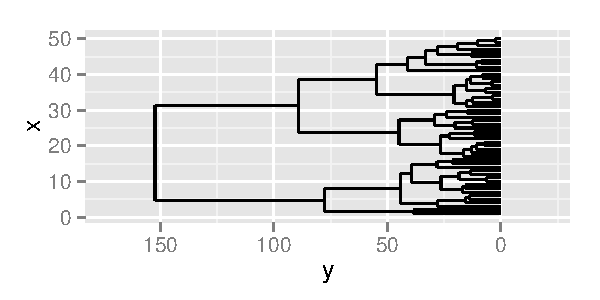
\includegraphics[width=4in, height=2in]{ggdendro-dendro1}
\end{center}
\caption{A dendrogram produced using \dendrodata{} and \code{ggplot()}}
\end{figure}


Of course, using ggplot to create the dendrogram means one has full control over the appearance of the plot.  For example, here is the same data, but this time plotted horizontally with a clean background:

\begin{Schunk}
\begin{Sinput}
> p <- p + coord_flip() +
+   opts(
+     panel.grid.major = theme_blank(),
+     panel.grid.minor = theme_blank(),
+     panel.background = theme_blank(),
+     axis.title.x = theme_text(colour=NA),
+     axis.title.y = theme_blank(),
+     axis.text.x = theme_blank(),
+     axis.text.y = theme_blank(),
+     axis.line = theme_blank()
+     )  
> print(p)
\end{Sinput}
\end{Schunk}

\begin{figure}[h]
\begin{center}
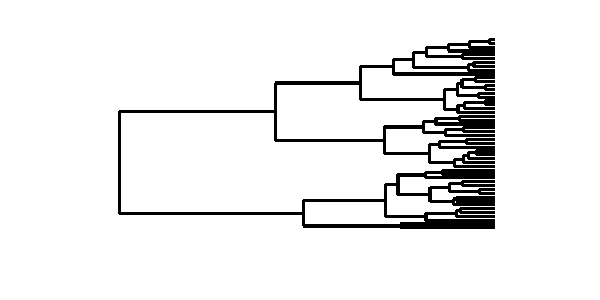
\includegraphics[width=4in, height=2in]{ggdendro-dendro2}
\end{center}
\caption{Dendrogram rotated on clear background}
\end{figure}

Dendrograms can also be drawn using triangular lines instead of rectangular lines.  For example:

\begin{Schunk}
\begin{Sinput}
> ddata <- dendro_data(dhc, type="triangle")
> p <- ggplot(segment(ddata)) + 
+     geom_segment(aes(x=x0, y=y0, xend=x1, yend=y1)) + 
+     coord_flip() + scale_y_reverse(expand=c(0.2, 0)) +
+     opts(
+         panel.grid.major = theme_blank(),
+         panel.grid.minor = theme_blank(),
+         panel.background = theme_blank(),
+         axis.title.x = theme_text(colour=NA),
+         axis.title.y = theme_blank(),
+         axis.text.x = theme_blank(),
+         axis.text.y = theme_blank(),
+         axis.line = theme_blank()
+     )  
> print(p)
\end{Sinput}
\end{Schunk}

\begin{figure}[h]
\begin{center}
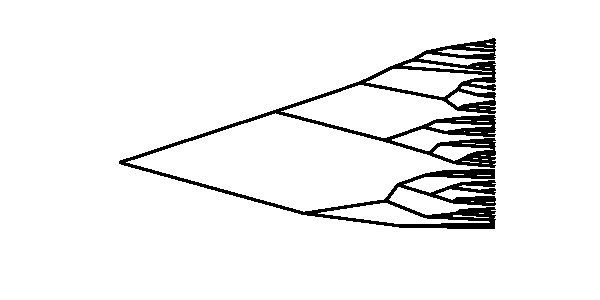
\includegraphics[width=4in, height=2in]{ggdendro-dendro3}
\end{center}
\caption{A dendrogram with triangular connection lines}
\end{figure}

  

\section{Tree diagrams}

The \code{tree} function in package \code{tree} creates tree diagrams.  To extract the plot data for these diagrams using \ggdendro{} follows the same basic pattern as dendrograms: 

\begin{Schunk}
\begin{Sinput}
> require(tree)
> data(cpus, package="MASS")
> cpus.ltr <- tree(log10(perf) ~ syct+mmin+mmax+cach+chmin+chmax, cpus)
> tree_data <- dendro_data(cpus.ltr)
> p <- ggplot(segment(tree_data)) +
+     geom_segment(aes(x=x, y=y, xend=xend, yend=yend, size=n), 
+         colour="blue", alpha=0.5) +
+     scale_size("n", to=c(0, 3)) +
+     geom_text(data=label(tree_data), 
+         aes(x=x, y=y, label=label), vjust=-0.5, size=3) +
+     geom_text(data=leaf_label(tree_data), 
+         aes(x=x, y=y, label=label), vjust=0.5, size=2)
> print(p)
\end{Sinput}
\end{Schunk}

\begin{figure}[h]
\begin{center}
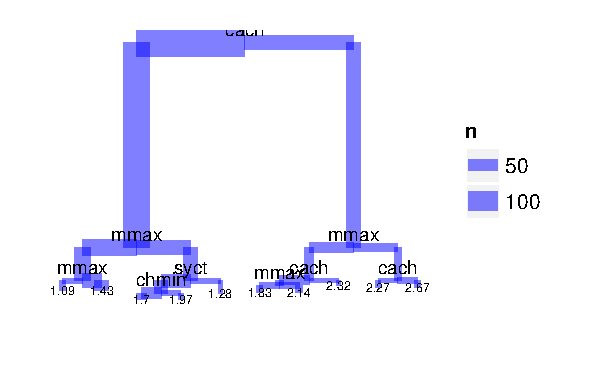
\includegraphics[width=4in, height=3in]{ggdendro-tree1}
\end{center}
\caption{Tree plot}
\end{figure}


\section{Conclusion}

The \ggdendro{} package makes it easy to extract the line segment and label data from hclust, dendrogram and tree objects.


% Start a new page
% Not echoed, not evaluated
% ONLY here for checkVignettes so that all output doesn't
% end up on one enormous page

\end{document}




